\subsection{Elenco dei casi d'uso - Utente: sviluppatore}	\subsubsection{UC-15 Ricerca dei dati delle annotazioni}	
		\begin{itemize}
			\item \textbf{Attori:} Sviluppatore.
			\item \textbf{Precondizione:} Lo sviluppatore si trova nella vista principale dell'applicazione.
			\item \textbf{Postcondizione:} Lo sviluppatore ottiene una lista delle annotazioni correnti delle frasi.
			\item \textbf{Scenario principale:}
				\begin{enumerate}
					\item Lo sviluppatore accede all'area dei dati.
					\item Lo sviluppatore scrive nella barra di ricerca una sottostringa della frase cercata (possibilmente nulla).
					\item (UC-15.1) lo sviluppatore seleziona i filtri da usare nella ricerca (possibilmente nessuno).
				\end{enumerate}
		\end{itemize}
	
	\subsubsection{UC-15.1 Filtraggio dei dati}	
		\begin{itemize}
			\item \textbf{Attori:} Sviluppatore.
			\item \textbf{Precondizione:} Lo sviluppatore si trova nell'area dati e ha scritto nella barra di ricerca una sottostringa della frase cercata.
			\item \textbf{Postcondizione:} Lo sviluppatore ottiene una lista di frasi in base al filtro selezionato.
			\item \textbf{Scenario principale:}
				\begin{enumerate}
					\item Lo sviluppatore seleziona il filtro su base temporale (UC-15.1.1).
					\item Lo sviluppatore seleziona il filtro in base agli utenti (UC-15.1.2).
					\item Lo sviluppatore indica dei parametri per restringere la ricerca.
					\item Lo sviluppatore esegue la ricerca.
				\end{enumerate}	
			\item \textbf{Estensioni:}
				\begin{itemize}
					\item 4.a Se i parametri inseriti dall'utente non sono coerenti viene mostrato un messaggio di errore (UC-5).
				\end{itemize}		
		\end{itemize}
	\begin{figure}[h]
			\centering
			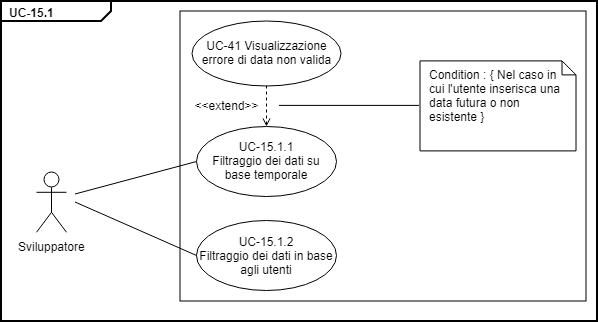
\includegraphics[scale=0.7]{images/UC-15_1.png}
			\caption{UC-15.1 Filtraggio dei dati}
		\end{figure}	
	
	\subsubsection{UC-15.1.1 Filtraggio dei dati su base temporale}	
		
		\begin{itemize}
			\item \textbf{Attori:} Sviluppatore.
			\item \textbf{Precondizione:} Lo sviluppatore si trova nell'area dati e ha scritto nella barra di ricerca una sottostringa della frase cercata.
			\item \textbf{Postcondizione:} Lo sviluppatore ottiene una lista di frasi in base al range temporale indicato.
			\item \textbf{Scenario principale:}
				\begin{enumerate}
					\item Lo sviluppatore seleziona il filtro.
					\item Lo sviluppatore indica due date che definiscono un intervallo di tempo per restringere la ricerca.
				\end{enumerate}
		\end{itemize}	
	\begin{figure}[h]
			\centering
			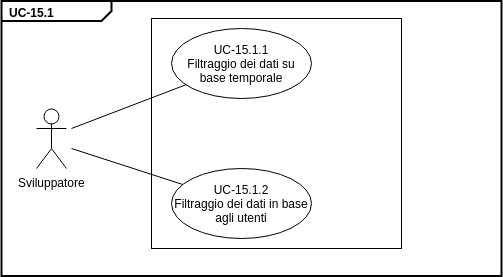
\includegraphics[scale=0.7]{images/UC-15_1_1.png}
			\caption{UC-15.1.1 Filtraggio dei dati su base temporale e UC-15.1.2 Filtraggio dei dati in base agli utenti}
		\end{figure}	
				
	\subsubsection{UC-15.1.2 Filtraggio dei dati in base agli utenti}	
		\begin{itemize}
			\item \textbf{Attori:} Sviluppatore.
			\item \textbf{Precondizione:} Lo sviluppatore si trova nell'area dati e ha scritto nella barra di ricerca una sottostringa della frase cercata.
			\item \textbf{Postcondizione:} Lo sviluppatore ottiene una lista di frasi in base agli utenti scelti.
			\item \textbf{Scenario principale:}
				\begin{enumerate}
					\item Lo sviluppatore seleziona il filtro (inclusione o esclusione di un utente).
					\item Lo sviluppatore indica l'utente (o la lista di utenti).
					\item Lo sviluppatore esegue la ricerca.
				\end{enumerate}
		\end{itemize}	
	\subsubsection{UC-16 Visualizzazione dei dati di una annotazione di una frase}
		\begin{itemize}
			\item \textbf{Attori:} Sviluppatore.
			\item \textbf{Precondizione:} Lo sviluppatore si trova nell'area dati e ha a disposizione i risultati della ricerca delle annotazioni.
			\item \textbf{Postcondizione:} Lo sviluppatore legge i dati di una annotazione di una frase.
			\item \textbf{Scenario principale:}
				\begin{enumerate}
					\item Lo sviluppatore sceglie una annotazione.
				\end{enumerate}
		\end{itemize}
	
	\subsubsection{UC-17 Visualizzazione storico}		
		\begin{itemize}
			\item \textbf{Attori:} Sviluppatore.
			\item \textbf{Precondizione:} Lo sviluppatore si trova nell'area dati e ha a disposizione i risultati della ricerca delle annotazioni.
			\item \textbf{Postcondizione:} Lo sviluppatore ottiene lo storico delle annotazioni ottenuta nella ricerca precedente.
			\item \textbf{Scenario principale:}
			\begin{enumerate}
				\item Lo sviluppatore seleziona l'opzione "vedi storico".
			\end{enumerate}
		\end{itemize}
\begin{figure}[h]
			\centering
			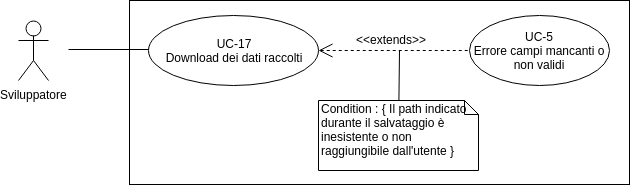
\includegraphics[scale=0.7]{images/UC-17.png}
			\caption{UC-17 Visualizzazione storico}
		\end{figure}		
		
	\subsubsection{UC-18 Ordinamento dei risultati}
		\begin{itemize}
			\item \textbf{Attori:} Sviluppatore.
			\item \textbf{Precondizione:} Lo sviluppatore si trova nell'area dati con i risultati della ricerca effettuata.
			\item \textbf{Postcondizione:} Lo sviluppatore ottiene la lista precedente ordinata in base alle scelte effettuate.
			\item \textbf{Scenario principale:}
				\begin{enumerate}
					\item Lo sviluppatore sceglie il parametro secondo il quale ordinare i risultati (frase, frequenza, ultima correzione, utente).
					\item Lo sviluppatore richiede l'ordinamento scelto.
				\end{enumerate}
		\end{itemize} 
	
	\subsubsection{UC-19 Download dei dati raccolti}
		\begin{itemize}
			\item \textbf{Attori:} Sviluppatore.
			\item \textbf{Precondizione:} Lo sviluppatore si trova nell'area dati con i risultati della ricerca effettuata.
			\item \textbf{Postcondizione:} Lo sviluppatore ottiene un file con i dati dei risultati precedentemente trovati.
			\item \textbf{Scenario principale:}
				\begin{enumerate}
					\item Lo sviluppatore richiede il download dei dati.
					\item Lo sviluppatore decide il path in cui il file viene salvato.
					\item Lo sviluppatore esegue il salvataggio.
				\end{enumerate}
			\item \textbf{Estensioni:}
				\begin{itemize}
					\item 2.a Se il path indicato è inesistente, viene visualizzato un messaggio di errore (UC-5).
				\end{itemize}
		\end{itemize} 


		
	\subsubsection{UC-20 Visualizzazione di un modello}
		\begin{itemize}
			\item \textbf{Attori:} Sviluppatore.
			\item \textbf{Precondizione:} Lo sviluppatore si trova nella vista principale dell'applicazione.
			\item \textbf{Postcondizione:} Lo sviluppatore ottiene le informazioni di un modello.
			\item \textbf{Scenario principale:}
			\begin{enumerate}
				\item Lo sviluppatore accede all'area modelli.
				\item Lo sviluppatore seleziona un modello.
			\end{enumerate}
	\end{itemize}
	
	\subsubsection{UC-21 Download di un modello}
			\begin{itemize}
			\item \textbf{Attori:} Sviluppatore.
			\item \textbf{Precondizione:} Lo sviluppatore si trova nella vista con le informazioni del modello selezionato.
			\item \textbf{Postcondizione:} Lo sviluppatore ottiene un file con il modello.
			\item \textbf{Scenario principale:}
			\begin{enumerate}
					\item Lo sviluppatore richiede il download del modello.
					\item Lo sviluppatore decide il path in cui il file viene salvato.
					\item Lo sviluppatore esegue il salvataggio.
				\end{enumerate}
			\item \textbf{Estensioni:}
				\begin{itemize}
					\item 2.a Se il path indicato è inesistente, viene visualizzato un messaggio di errore (UC-5).
				\end{itemize}
		\end{itemize}
\begin{figure}[h]
			\centering
			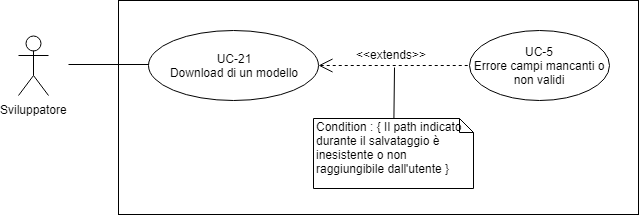
\includegraphics[scale=0.7]{images/UC-21.png}
			\caption{UC-21 Download di un modello}
		\end{figure}		
		
	\subsubsection{UC-22 Creazione di un modello}		
		\begin{itemize}
			\item \textbf{Attori:} Sviluppatore.
			\item \textbf{Precondizione:} Lo sviluppatore si trova nella vista principale dell'applicazione.
			\item \textbf{Postcondizione:} Lo sviluppatore aggiunge un modello alla piattaforma.
			\item \textbf{Scenario principale:}
			\begin{enumerate}
				\item Lo sviluppatore accede all'area modelli.
				\item Lo sviluppatore seleziona la funzione di aggiunta di un modello.
				\item Lo sviluppatore inserisce i dati per la creazione del modello.
				\item Lo sviluppatore completa la creazione.
			\end{enumerate}
			\item \textbf{Estensioni:}
				\begin{itemize}
					\item 4.a Se uno dei dati inseriti non è coerente, allora viene visualizzato un messaggio di errore (UC-5).
				\end{itemize}
		\end{itemize}
		
		\begin{figure}[h]
			\centering
			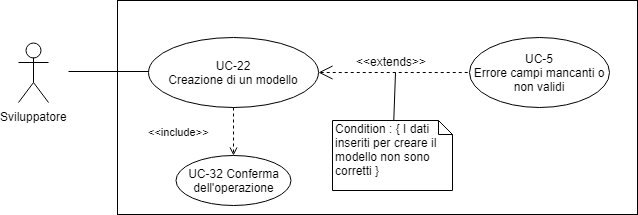
\includegraphics[scale=0.7]{images/UC-22.png}
				\caption{UC-22 Creazione di un modello}
		\end{figure}	
	